
\subsection{Off-Card Teil}
\label{subsec:3.3}

% der offcard Teil besteht aus der graphischen Oberfläche, der Logik zur Steuerung der Oberfäche und der Logik zur Kommunikation mit der Smartcard
%screenshots mit erklärungen was gemacht wird + grob technisches
%passwörter werden gehashed
%Packagediagramm

Der Inhalt dieses Abschnittes bildet die Umsetzung des Off-Card-Teils. Dabei wird auf die graphische Oberfläche, die Logik zur Steuerung und zur Kommunikation mit der Smartcard eingegangen. \\
\newline
Wenn man die Off-Card-Anwendung startet, gelangt man in das Hauptmenü der Anwendung, welches in der Abbildung \ref{main}  dargestellt ist. Dieses Menü enthält fünf Buttons, welche jeweils zu einer Funktion des Programmes führt. Den gesamten Trainingsplan, den Tagesplan und den Trainingsfortschritt kann man sich ohne Eingabe eines Passwortes anschauen. Um die Trainingsergebnisse einzutragen oder den Trainingsplan zu ändern, ist ein Passwort nötig. Jede der Funktionen, sowie die Passwortabfrage, wird im folgenden genauer erläutert.

\begin{figure}[h]
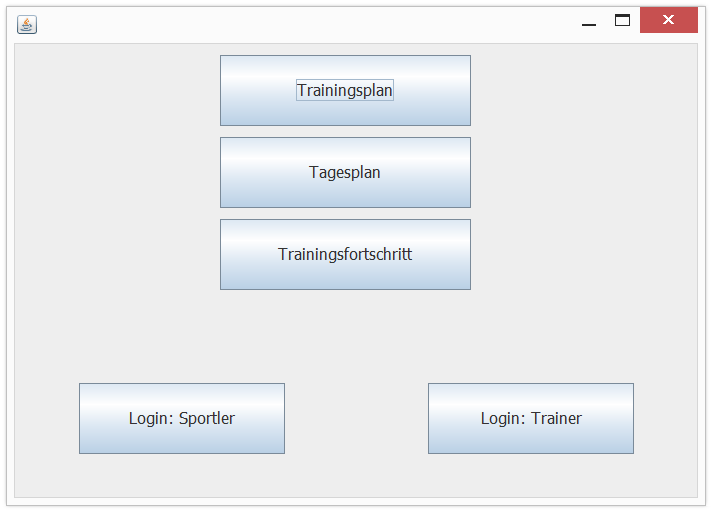
\includegraphics[width=1\hsize]{./images/main.png}
\caption{Hauptmenü}
\label{main}
\end{figure}



\subsubsection*{Trainingsplan}

Über den Button Trainingsplan gelangt man in die nächste Ansicht, welche den gesamten aktuellen Trainingsplan darstellt (Abb. \ref{main}). Um den Trainingsplan zu laden, ruft das Programm die Funktion CardInterface.getWorkoutplan() aus dem CardInterface auf, welche als Rückgabewert den aktuellen Trainingsplan liefert. Dieser wird im Anschluss ausgelesen und in die Tabelle geschrieben. Wenn der Trainingsplan leer ist, ist folglich auch die Tabelle leer. Über den Zurück Button gelangt man, wie auch in allen anderen Funktion, zurück in das Hauptmenü.

\begin{figure}[h]
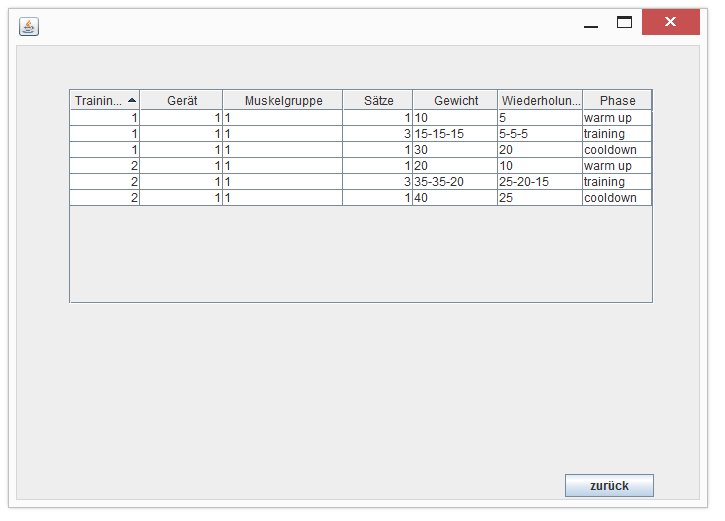
\includegraphics[width=1\hsize]{./images/gesamt.png}
\caption{gesamter Trainingsplan}
\label{main}
\end{figure}

\subsubsection*{Tagesplan}

Die Ansicht des Tagesplan ist ähnlich zur Anzeige des gesamten Trainingsplans, mit einer Einschränkung. Über die Combobox "'Tag"' kann der gewünschte Tag ausgewählt werden. Nach dieser Auswahl wird in der Tabelle, welche den Trainingsplan anzeigt, nur diejenigen Übungen eingetragen und dargestellt, welche an dem jeweiligen Tag ,laut Trainingsplan, stattfinden sollen. Dazu besitzt jede Stage in einem Workoutplan-Object ein Attribut day. Diese Ansicht ist in Abbildung \ref{day} zu sehen.

\begin{figure}[h]
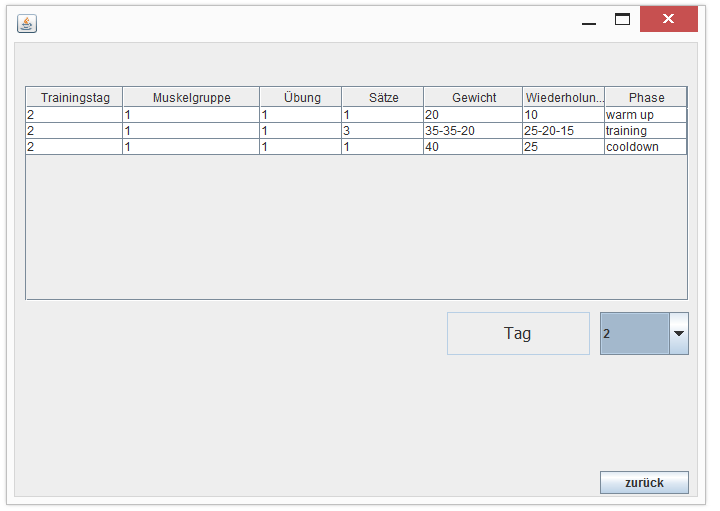
\includegraphics[width=1\hsize]{./images/tag.png}
\caption{Tagesplan}
\label{day}
\end{figure}
\newpage
\subsubsection*{Login: Trainer}

Um einen Trainingsplan mit den beiden Funktionen Trainingsplan und Tagesplan anzeigen zu können, ist es zuvor notwendig, einen Trainingsplan zu erzeugen. Dies ist möglich, wenn man sich als Trainer einloggt, wozu eine Passworteingabe nötig ist (Abb. \ref{login}).

\begin{figure}[h]
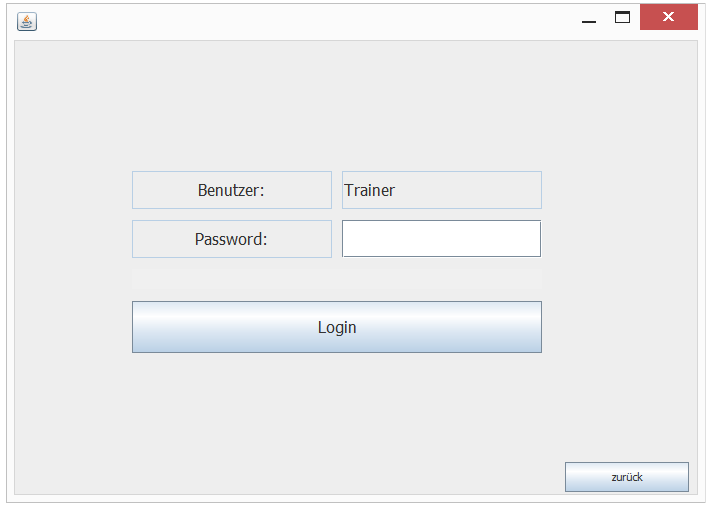
\includegraphics[width=1\hsize]{./images/login.png}
\caption{Eingabemenü des Trainers}
\label{login}
\end{figure}
\newpage
Wenn man sien Passwort eingegeben hat und auf Login drückt, wird das Passwort gehashed und an die Smartcard mit dem Benutzertyp (Trainer oder Sportler) gesendet. Diese überprüft das Passwort auf Korrektheit und gibt als Antwort true oder false zurück. Wenn das Passwort korrekt ist, gelangt man in die Traineransicht und kann den aktuellen Trainingsplan verändern oder einen neuen anlegen. Die Ansicht ist in Abbildung \ref{trainer} dargestellt. Über den Button neue Übung können weitere Zeilen zur Tabelle hinzugefügt werden. Zusätzlich zu den Übungen kann ein Start und Enddatum für diesen Trainingsplan festgelegt werden. Da auf der Karte keine Strings gespeichert werden können, muss man mit ID's arbeiten. Diese ID's kann man dann im Off-Card-Teil über eine Hashmap speziellen Strings zuweisen um beispielsweise die Muskelgruppe nicht, wie in der Abb. \ref{trainer} zu sehen ist, als Zahl darstellen zu müssen. Beim speichern des Trainingsplans wird die Tabelle ausgelesen und die entsprechenden Werte einem neuen Workoutplan-Objekt zugewiesen, welches auf der Smartcard gespeichert wird. Zusätzlich dazu wird, auch ein neues Progressarray auf der Karte erzeugt, welche alle Stage-ID's für den neuen Plan enthält. Dies ist notwendig um den Fortschritt des Sportlers eintragen, speichern und auslesen zu können.

\begin{figure}[h]
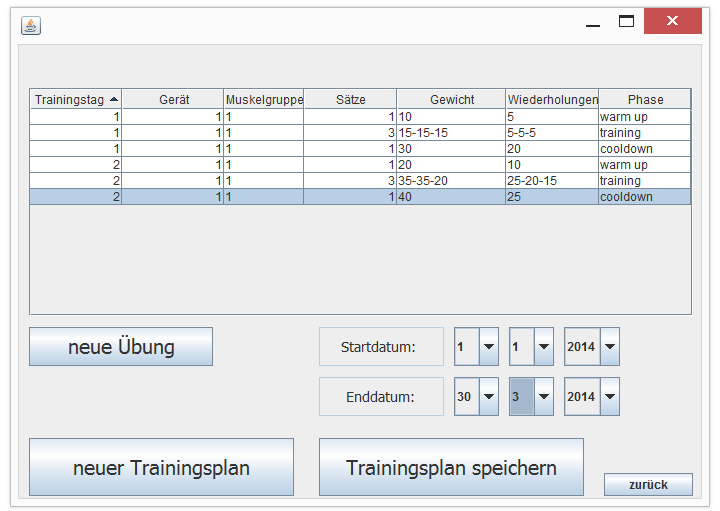
\includegraphics[width=1\hsize]{./images/Trainer.png}
\caption{Eingabemenü des Trainers}
\label{trainer}
\end{figure}



\subsubsection*{Login: Sportler}

Wenn nun ein Trainingsplan erzeugt und abgespeichert wurde, kann der Sportler seine Trainingsdaten bezüglich dieses Plans eintragen. Dazu ist es notwendig, das er sich als Sportler einloggt. Wenn der Benutzer als Sportler angemeldet ist, gelangt er in die Sportleransicht, welche in Abb. \ref{sportler} zu sehen ist. In dieser Ansicht werden alle Übungen, für den ausgewählten Tag, angezeigt. Die Auswahl geschieht nach dem gleichen Prinzip, welches auch in der Tagesplanansicht benutzt wird, siehe Abschnitt Tagesplan. Die Daten zu den jewieligen Übungen, kann der Nutzer manuell eingeben, oder die vorgegebenen Trainingswerte über die Checkbox übernehmen lassen. Wenn die Daten eingetragen sind und gespeichert werden (Button: Trainingsdaten speichern), wird das Progressarray aktualisiert. Dazu wird es zunächst von der Karte gelesen, dann Werte die eingetragenen Werte überprüft, ob gegebenenfalls ein neuer bester oder schlechtester Wert erreicht wurde. Nach der Aktualisierung wird das Progressarray wieder auf der Karte abgelegt. 

\begin{figure}[h]
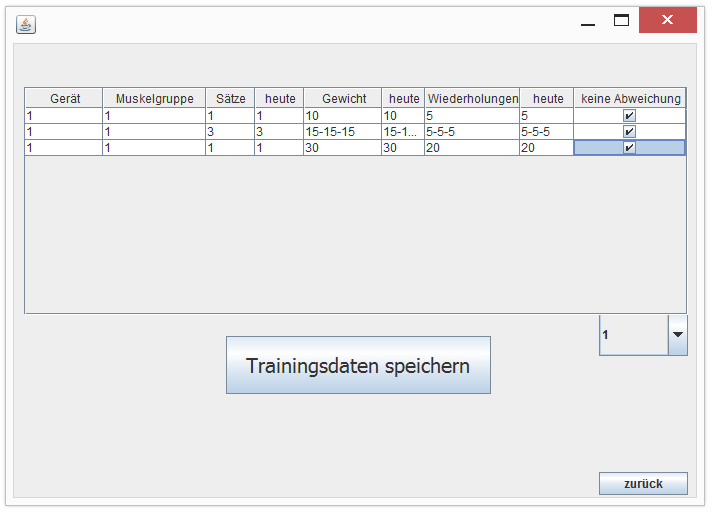
\includegraphics[width=1\hsize]{./images/sportler.png}
\caption{Eingabemenü des Sportlers}
\label{sportler}
\end{figure}
\newpage
\subsubsection*{Trainingsfortschritt}

Über die Funktion Trainingsfortschritt, kann wie es der Name sagt, sich den aktuellen Trainingsfortschritt anzeigen lassen. Dazu wird von der Karte der aktuelle Trainingsplan und das Progressarray abgerufen. Dabei gibt es verschiedene Möglichkeiten. Zum einen kann noch kein Trainingsplan existieren. Wenn dieser Fall vorliegt, bleibt die Tabelle leer und das Progressarray existiert folglich auch nicht und muss nicht ausgelesen werden. Wenn ein Trainingsplan existiert, allerdings noch keine Trainingsdaten eingetragen wurden, wird nur der Trainingsplan abgebildet und die Felder der Trainingsdaten bleiben leer, siehe Abb. \ref{empty}.

\begin{figure}[h]
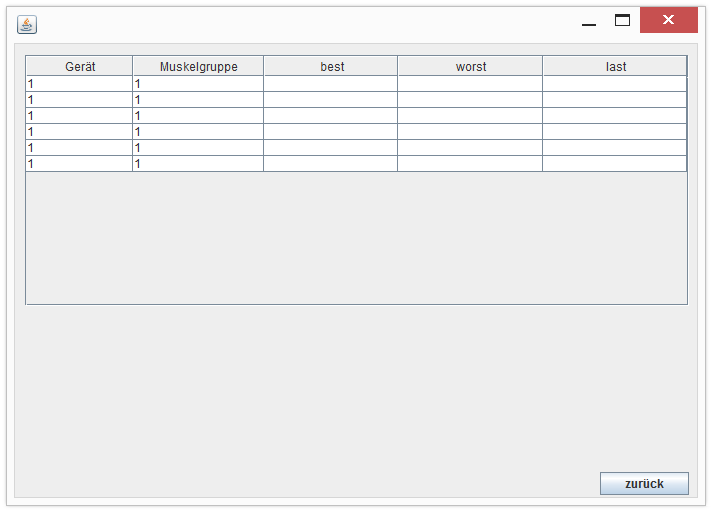
\includegraphics[width=1\hsize]{./images/fortschritt-leer.png}
\caption{Trainingsfortschritt ohne Einträge}
\label{empty}
\end{figure}
\newpage
Weiterhin exisitiert die Möglichkeit, das im Progressarray zu einigen Übungen schon Trainingsdaten vorhanden sind, allerdings noch nicht zu allen. Dann werden, wie in der Abbildung \ref{full} zu sehen ist, alle vorhandenen Werte eingetragen und die restlichen freigelassen. Die Spalte best bzw. worst gibt jeweils den besten bzw. schlechtesten Trainingswert an. Wenn ein neuer Trainingswert eingetragen wird, wird dieser immer in der Spalte last abgebildet. Um im späteren Verlauf nachvollziehen zu können, wann welcher Wert erreicht wurde, wird bezüglich der Daten noch ein Datum angegeben.

\begin{figure}[h]
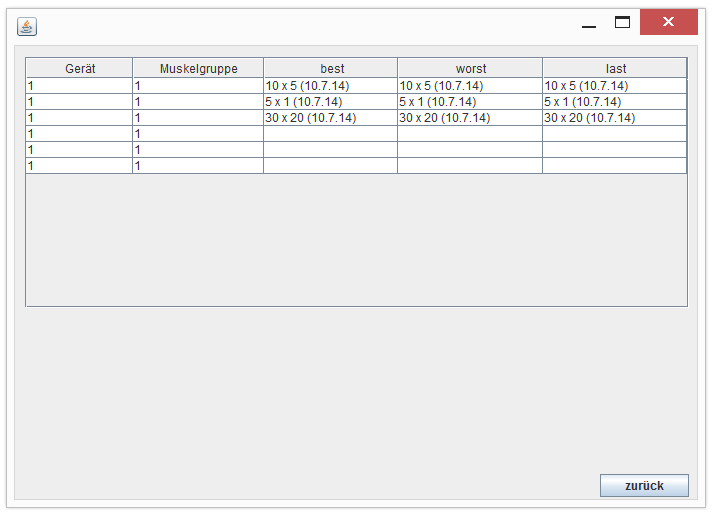
\includegraphics[width=1\hsize]{./images/fortschritt-mit-eingabe.png}
\caption{Trainingsfortschritt mit Einträgen}
\label{full}
\end{figure}
\newpage
\subsubsection*{Klassendiagramm Off-Card Teil}





\begin{figure}[h]
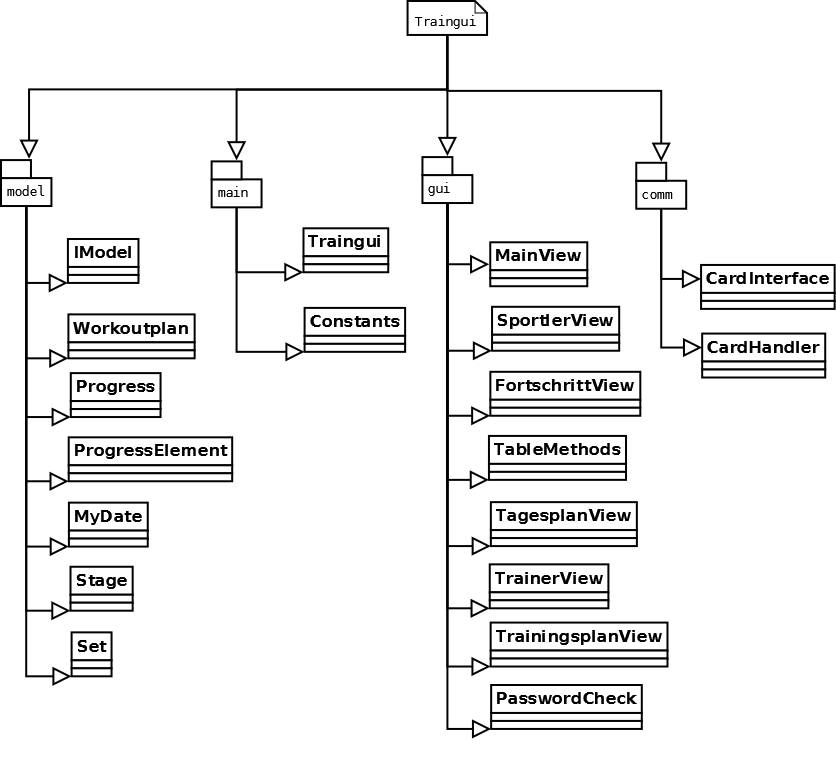
\includegraphics[width=1\hsize]{./images/Diagramm1.png}
\caption{Klassendiagramm Off-Card Teil}
\label{off-card}
\end{figure}

